%%%%%%%%%%%%%%%%%%%%%%%%%%%%%%%%%%%%%%%%%
% University Assignment Title Page 
% LaTeX Template
% Version 1.0 (27/12/12)
%
% This template has been downloaded from:
% http://www.LaTeXTemplates.com
%
% Original author:
% WikiBooks (http://en.wikibooks.org/wiki/LaTeX/Title_Creation)
%
% License:
% CC BY-NC-SA 3.0 (http://creativecommons.org/licenses/by-nc-sa/3.0/)
% 
% Instructions for using this template:
% This title page is capable of being compiled as is. This is not useful for 
% including it in another document. To do this, you have two options: 
%
% 1) Copy/paste everything between \begin{document} and \end{document} 
% starting at \begin{titlepage} and paste this into another LaTeX file where you 
% want your title page.
% OR
% 2) Remove everything outside the \begin{titlepage} and \end{titlepage} and 
% move this file to the same directory as the LaTeX file you wish to add it to. 
% Then add \documentclass[12pt]{article}
\usepackage[english]{babel}
\usepackage{amsmath}
\usepackage{graphicx}
\usepackage{textcomp}
\usepackage{parskip}
\usepackage[colorinlistoftodos]{todonotes}
\usepackage{csquotes}
\usepackage{float}
\usepackage[backend=biber,style=ieee]{biblatex}
\addbibresource{bibliography.bib}

\begin{document}

\begin{titlepage}

\newcommand{\HRule}{\rule{\linewidth}{0.5mm}}
\center 

\textsc{\LARGE Iowa State University }\\[1.5cm] 
\textsc{\Large Center for Statistics and Applications in Forensic
Evidence
}\\[0.5cm] 

\HRule \\[0.4cm]
{ \huge \bfseries Shoe Print Data Collection Phase 1 }\\[0.4cm] 
\HRule \\[1.5cm]



\begin{center}
\centering
\includegraphics[scale=.4]{csafe-logo}\\[1cm]
\end{center}







\end{titlepage}

\section{Introduction}

This manual was developed by researchers with the Center for Statistics and Applications in Forensic Evidence. Within it are the procedures that should be followed when collecting data for phase one of the longitudinal shoe impression study. If at any time there is a question on any of these procedures, please make a note using a post-it note and e-mail the principal investigator, the project  manager,  the  faculty  in  charge  of  the  study,  or  the  author  of  the specific procedure.


\end{document} to your LaTeX file where you want your
% title page.
%
%%%%%%%%%%%%%%%%%%%%%%%%%%%%%%%%%%%%%%%%%
%\title{Title page with logo}
%----------------------------------------------------------------------------------------
%	PACKAGES AND OTHER DOCUMENT CONFIGURATIONS
%----------------------------------------------------------------------------------------

\documentclass[12pt]{article}
\usepackage[english]{babel}
\usepackage[utf8x]{inputenc}
\usepackage{amsmath}
\usepackage{graphicx}
\usepackage[colorinlistoftodos]{todonotes}

\begin{document}

\begin{titlepage}

\newcommand{\HRule}{\rule{\linewidth}{0.5mm}} % Defines a new command for the horizontal lines, change thickness here

\center % Center everything on the page
 
%----------------------------------------------------------------------------------------
%	HEADING SECTIONS
%----------------------------------------------------------------------------------------

\textsc{\LARGE Iowa State University}\\[1.5cm] % Iowa State University 
\textsc{\Large CSAFE}\\[0.5cm] % CSAFE
\textsc{\large Center for Statistics and Applications in Forensic Evidence }\\[0.5cm] % Center for Statistics and Applications in Forensic Evidence 

%----------------------------------------------------------------------------------------
%	2D Shoe Scanner Procedure
%----------------------------------------------------------------------------------------

\HRule \\[0.4cm]
{ \huge \bfseries Vinyl Photo: Procedure }\\[0.4cm] % Title of your document
\HRule \\[1.5cm]
 
%----------------------------------------------------------------------------------------
%	AUTHOR SECTION
%----------------------------------------------------------------------------------------

\begin{minipage}{0.4\textwidth}
\begin{flushleft} \large
\emph{Author:}\\
James \textsc{E. Kruse} % Author
\end{flushleft}
\end{minipage}
~
\begin{minipage}{0.4\textwidth}
\begin{flushright} \large
\emph{Supervisor:} \\
Dr. Guillermo \textsc{Basulto-Elias} % Supervisor's Name
\end{flushright}
\end{minipage}\\[2cm]

% If you don't want a supervisor, uncomment the two lines below and remove the section above
%\Large \emph{Author:}\\
%John \textsc{Smith}\\[3cm] % Your name

%----------------------------------------------------------------------------------------
%	DATE SECTION
%----------------------------------------------------------------------------------------

{\large \today}\\[2cm] % Date, change the \today to a set date if you want to be precise

%----------------------------------------------------------------------------------------
%	LOGO SECTION
%----------------------------------------------------------------------------------------


 
%----------------------------------------------------------------------------------------

\vfill % Fill the rest of the page with whitespace

\end{titlepage}




\section{Introduction}

This is a continuation of the Paper Print/Vinyl Print Procedure. The following is the recommended procedure taking Vinyl Print photos.

\subsection{Procedure}

1. In the marked off area, position the flooring and the lights on the pre-laid spike tape. Position the ruler in the photo for scale. 

\begin{figure}[!htp]
\centering
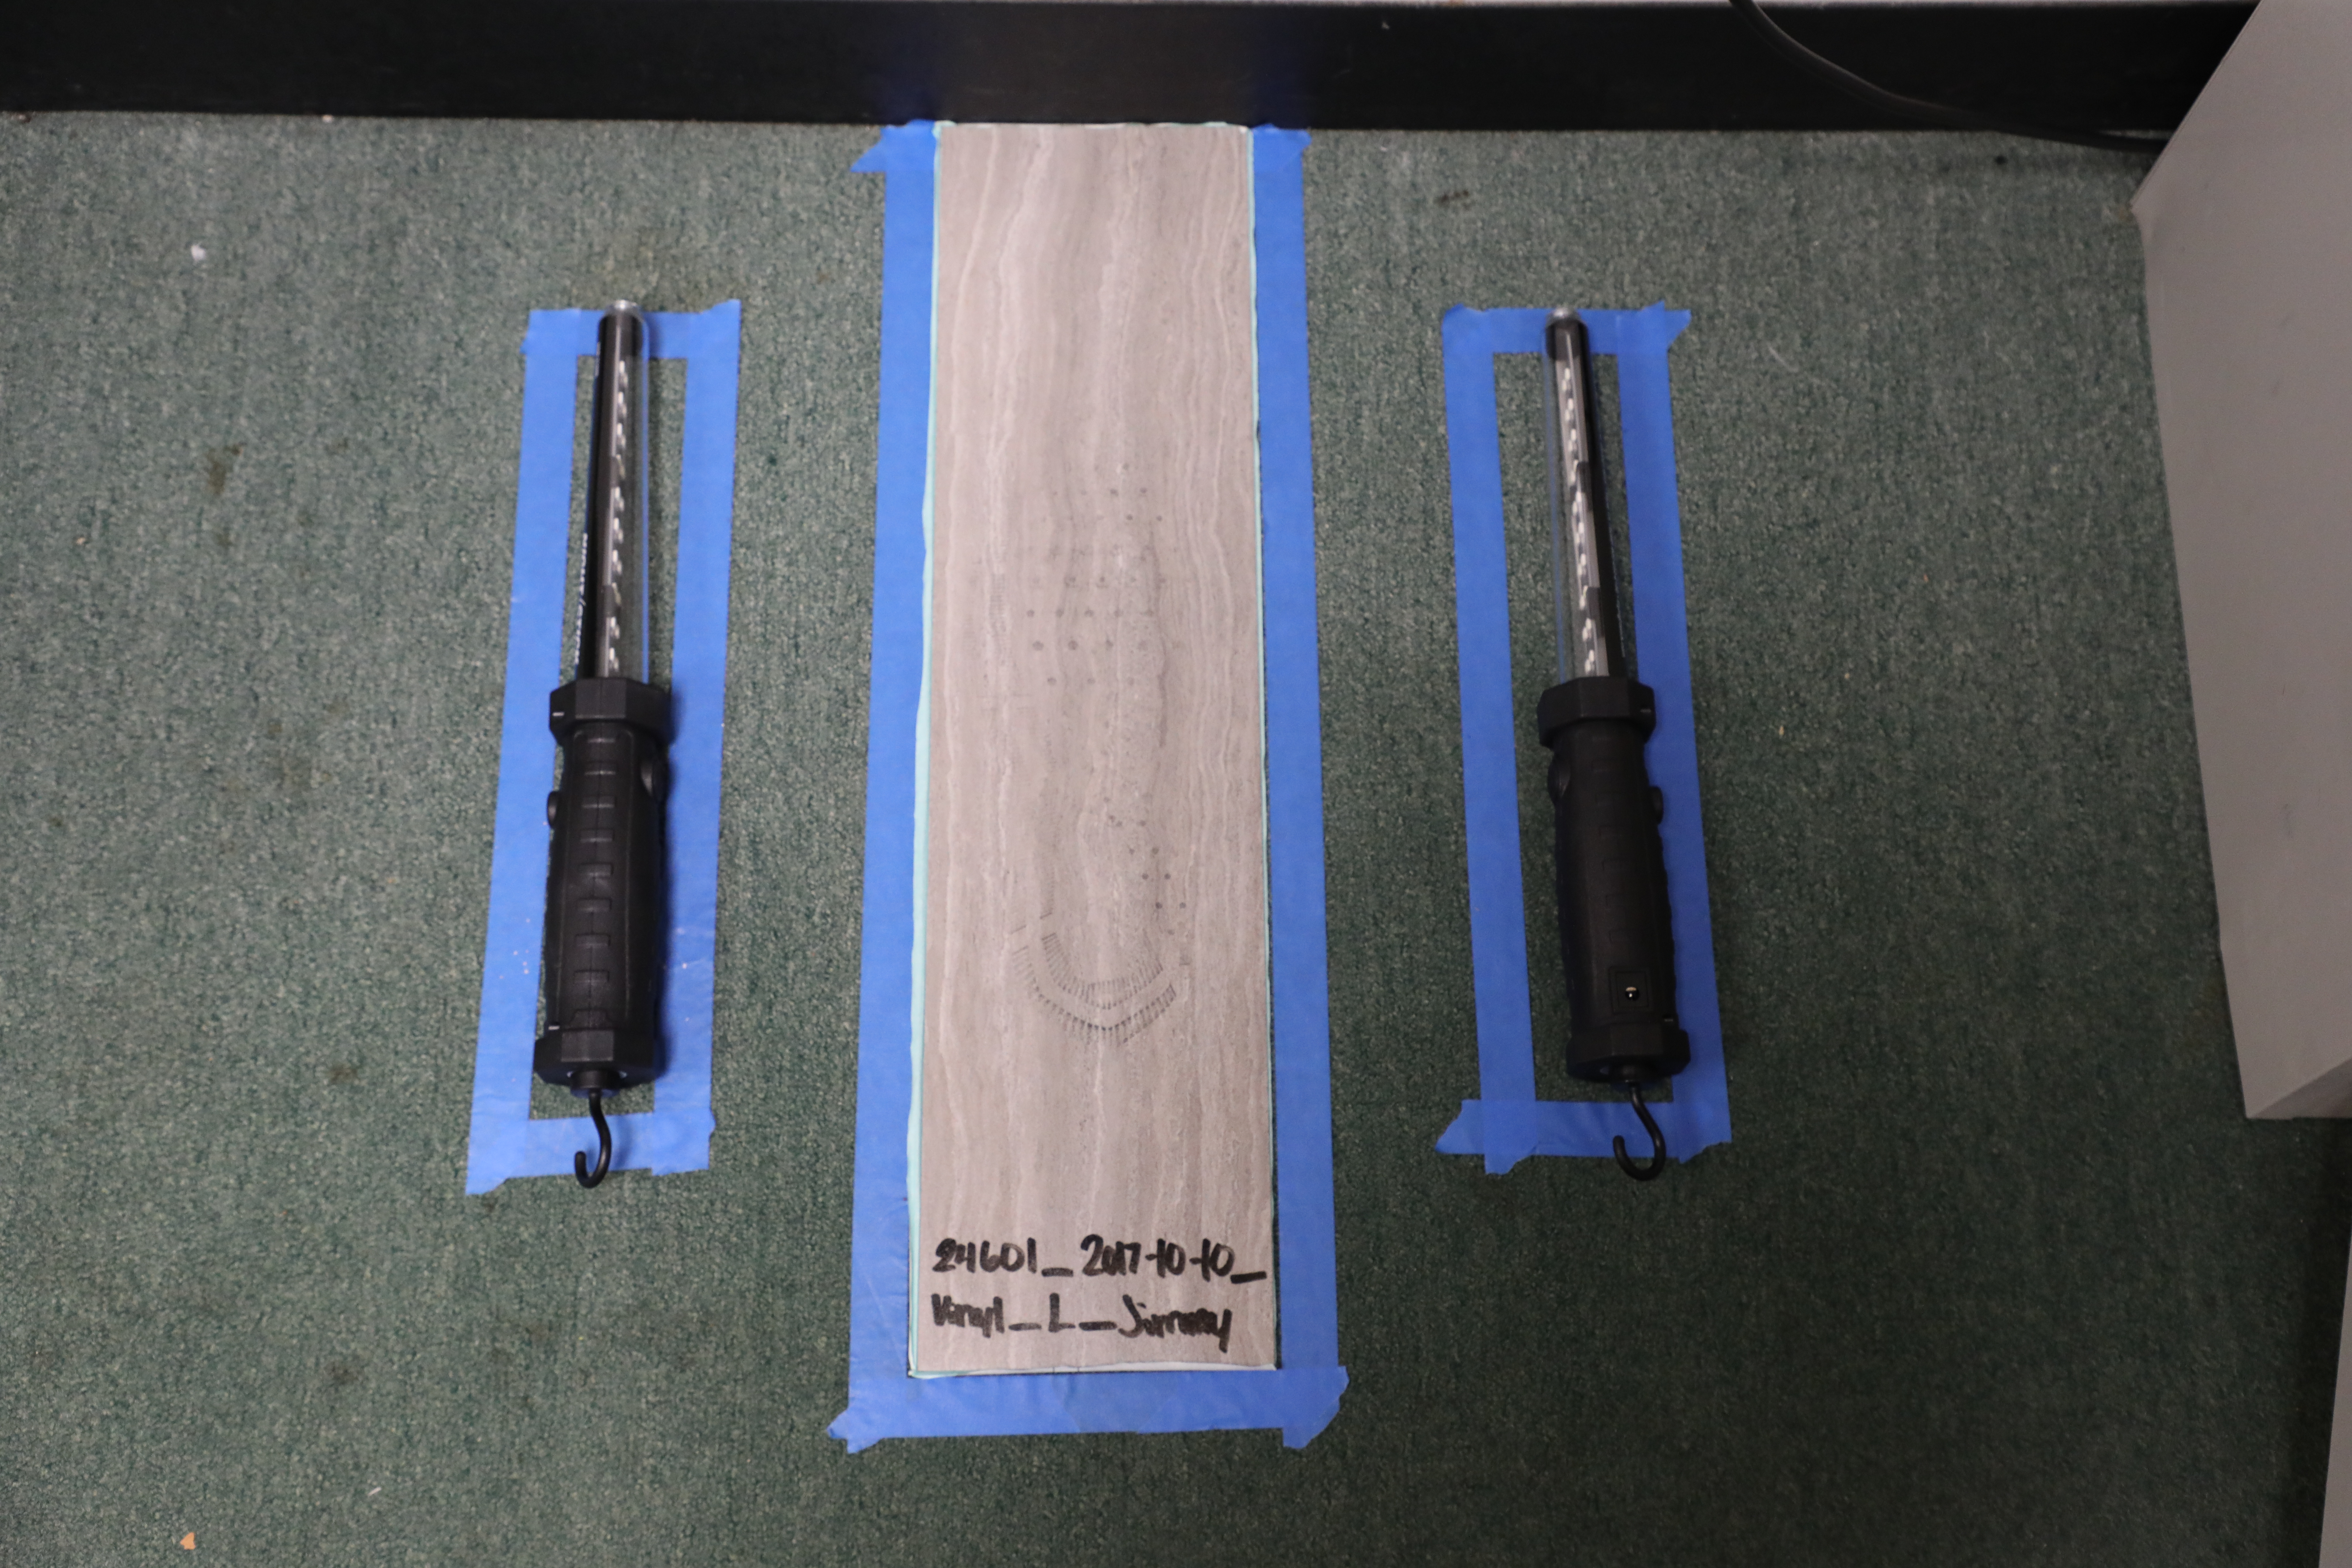
\includegraphics[scale=0.05]{Set}
\caption{Vinyl print set up.}
\label{img:Set}
\end{figure}

\begin{figure}[!htp]
\centering
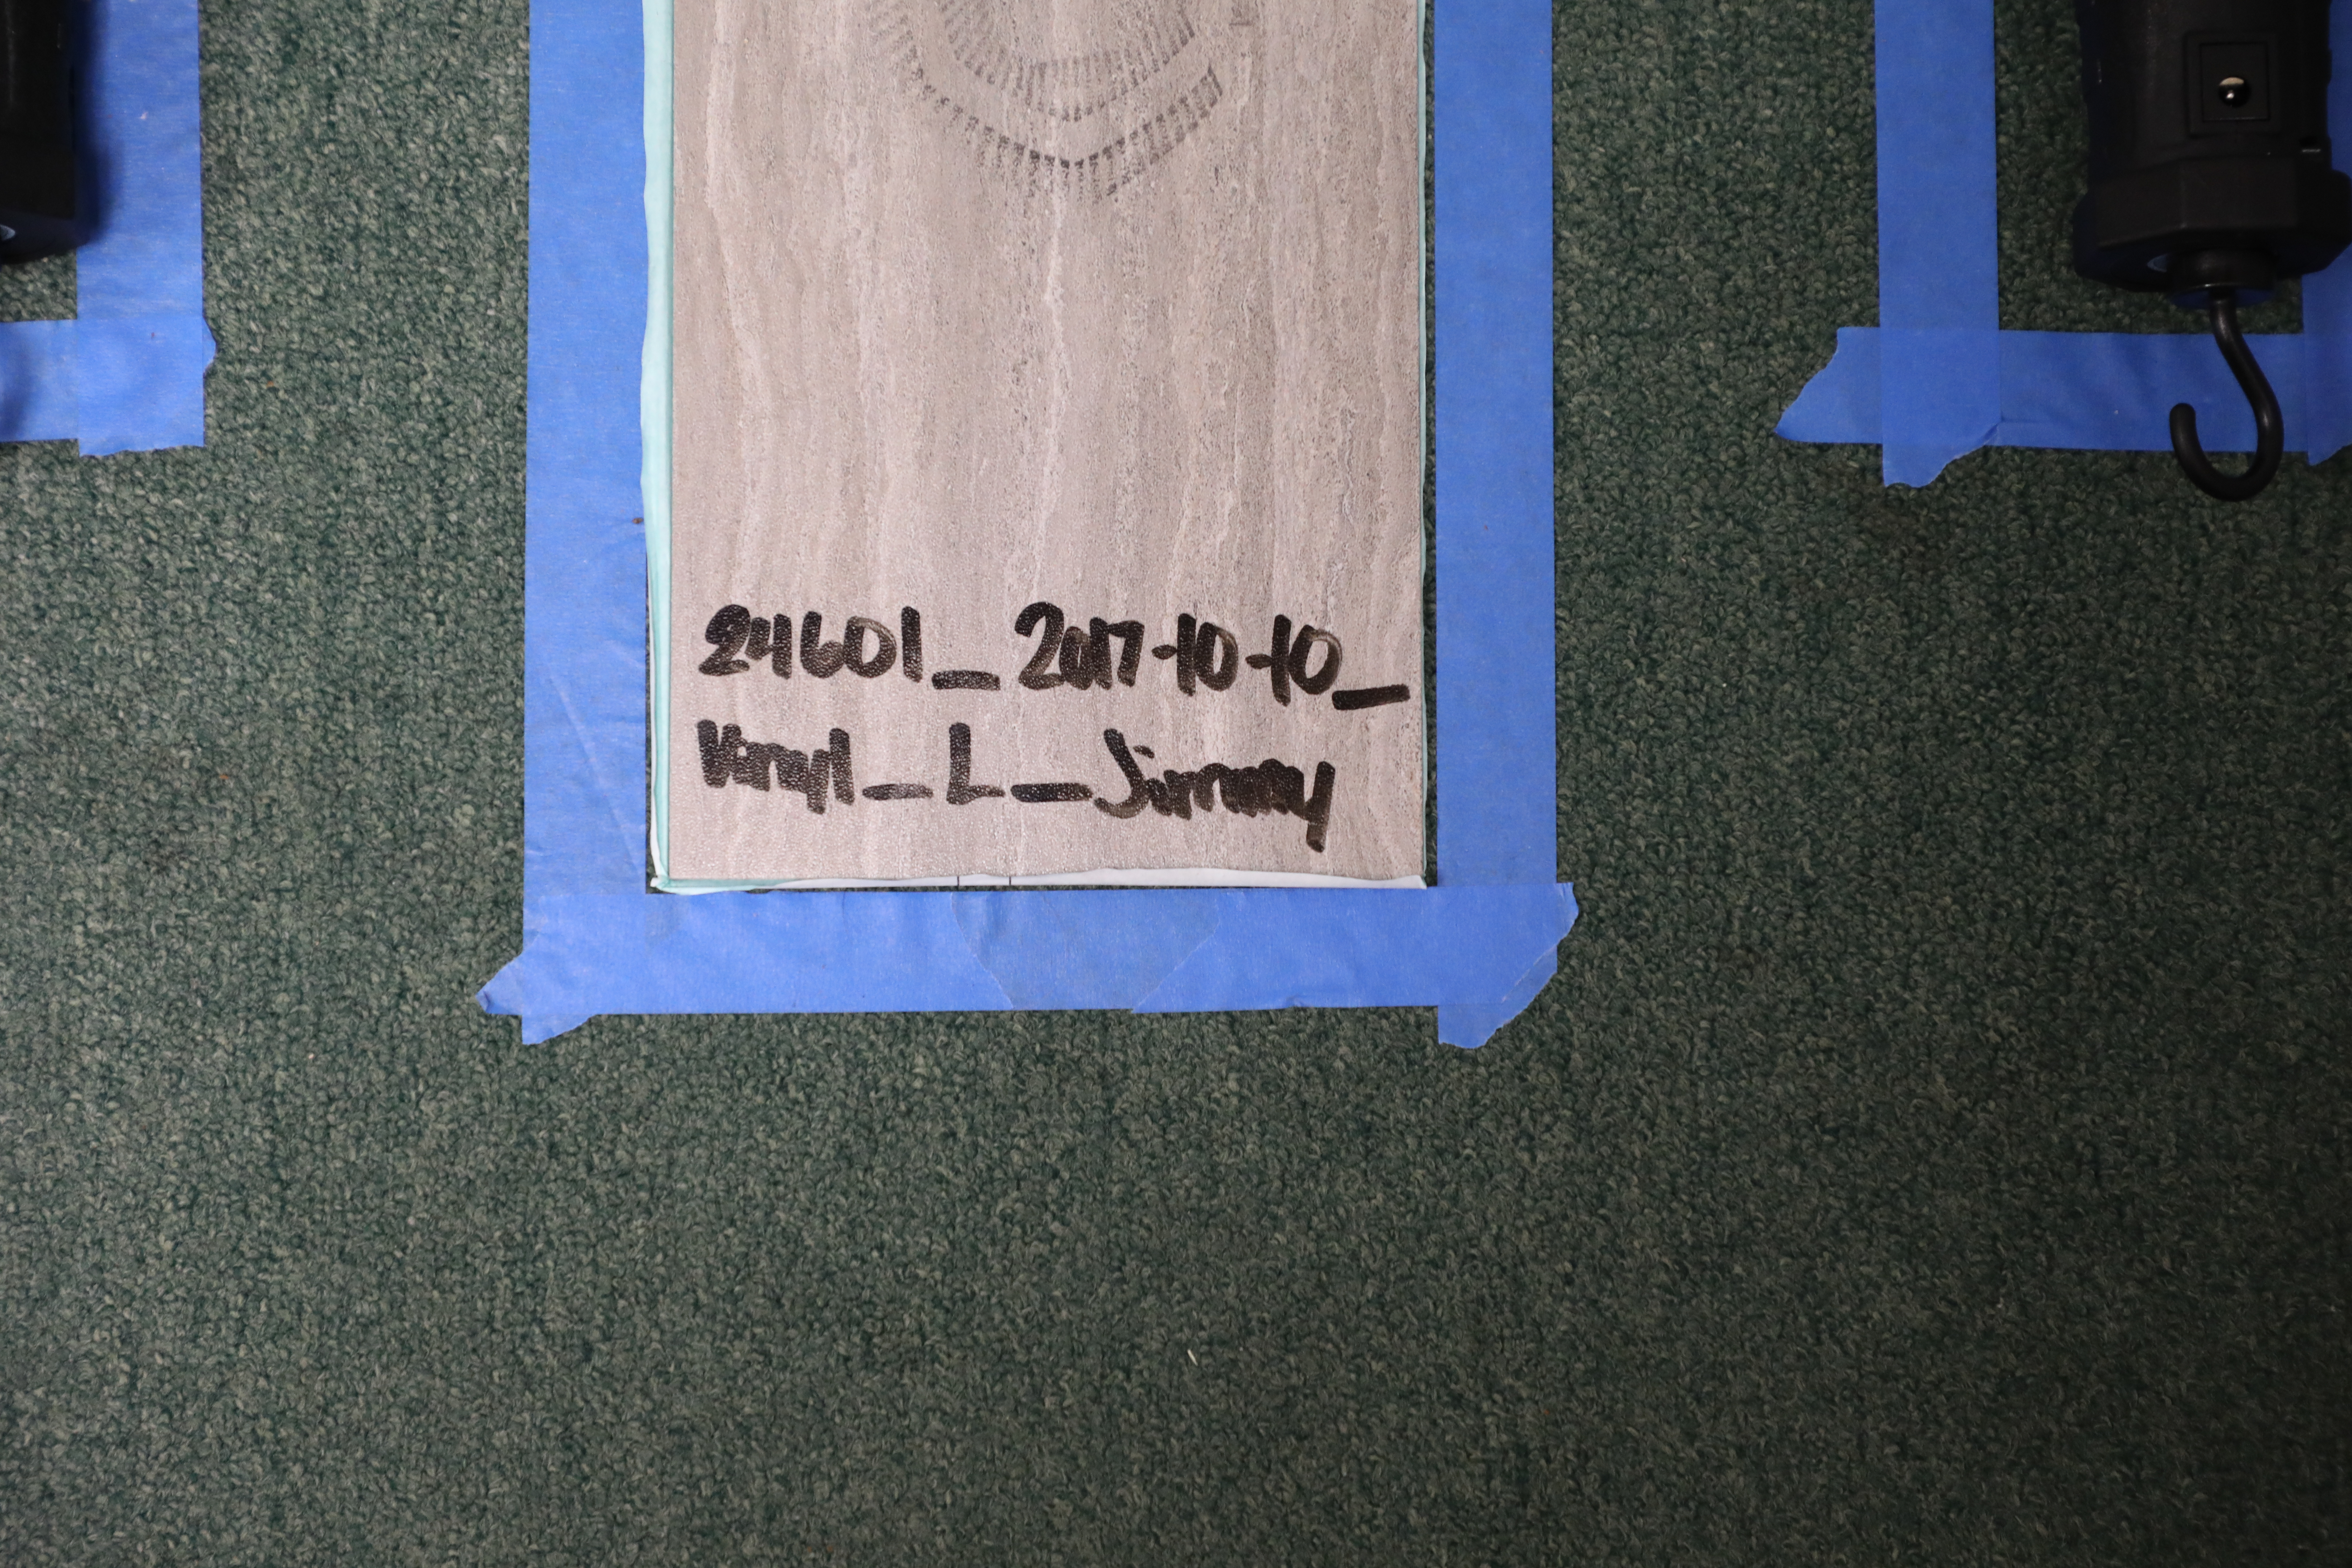
\includegraphics[scale=0.05]{Set2}
\caption{Label.}
\label{img:set2}
\end{figure}

2. Retrieve the camera and turn it on/make sure that the lens cap is removed. Turn off computer monitors, shut the door, and turn off the lights. Place a note on the door asking people to knock and wait outside if they need you. This will make sure that light dose not effect the photos.

3. Standing overhead of the print, take a photo straight down as if at a crime scene. The camera should be zoomed in on the full print even if the toe or heel is not completely visible. The lights should be positioned as they are in the example images (do not use the flash. Take multiple if needed and the best will be selected when reviewing the images. (Note: the label written in dry erase marker must be visible in the photo.) 

\begin{figure}[!htp]
\centering
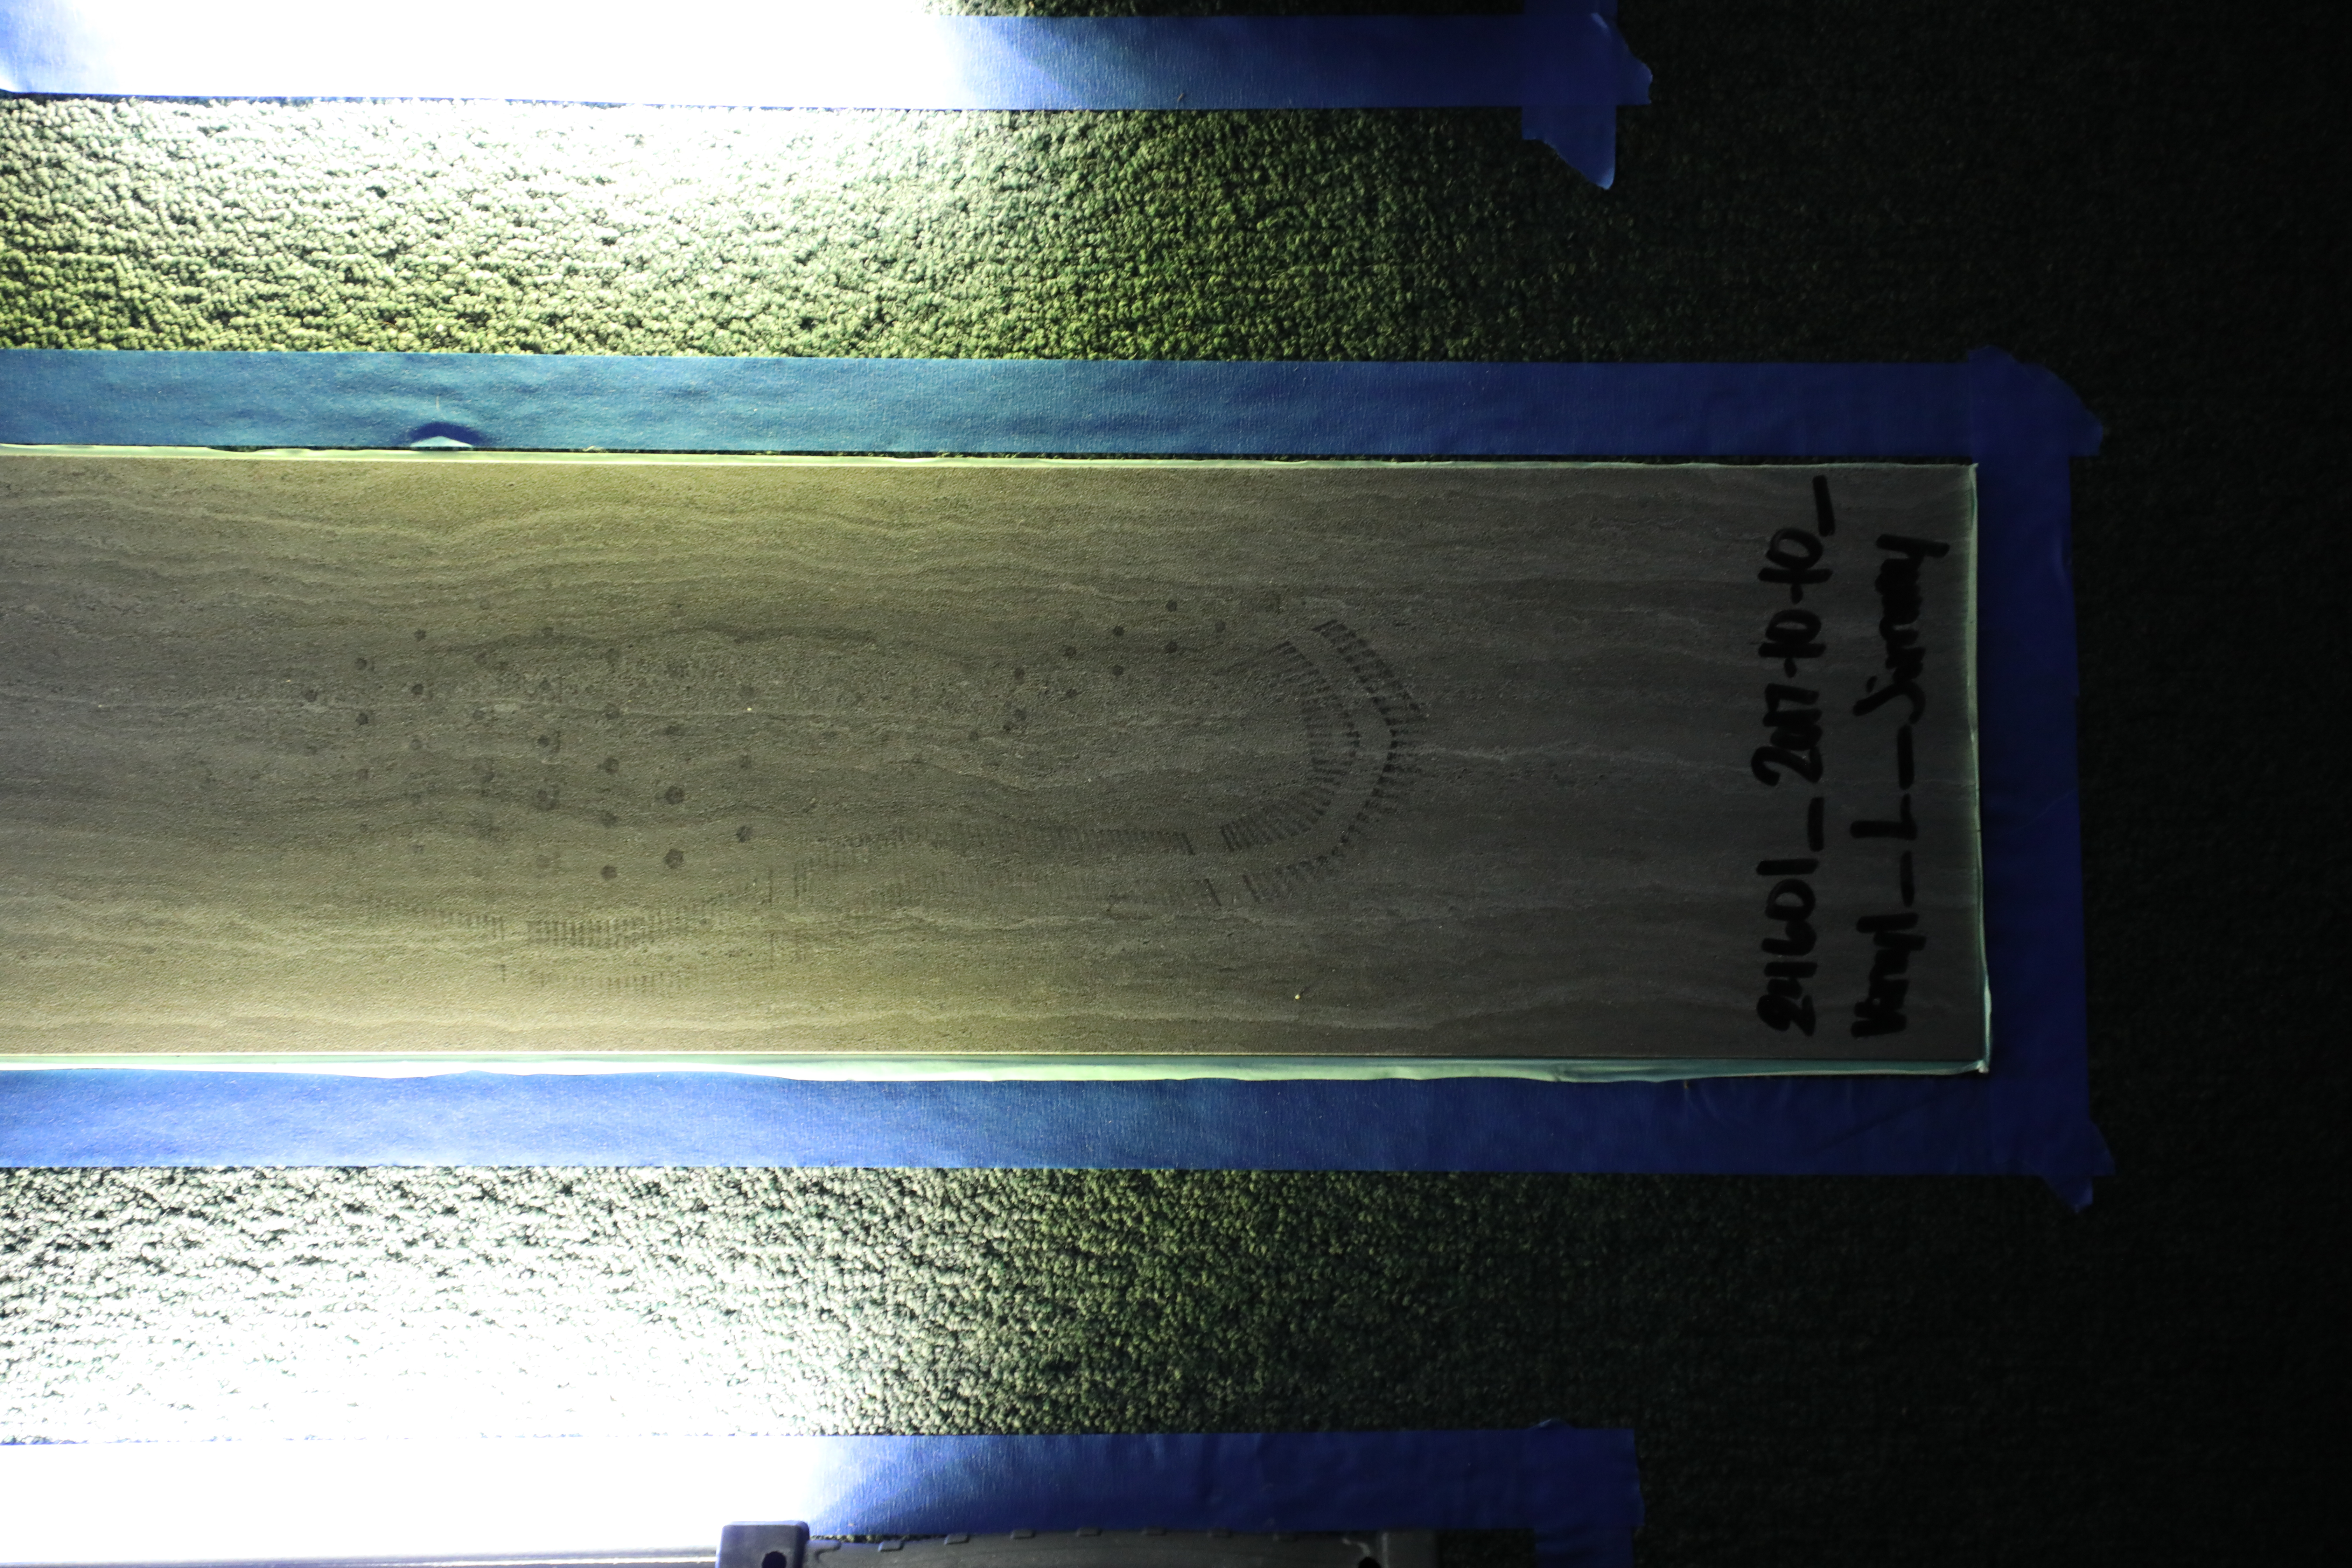
\includegraphics[scale=0.05]{Test}
\caption{Sample Photo.}
\label{img:Test}
\end{figure}

4. For the second rep., alter the name written in marker to account for the second image making sure not to damage the print. Take a second photo using the same procedure as above. 

5. Once all photos have been taken, compleatly clean the print and name off of the vinyl and allow to dry. 


6. For uploading these photos, please see the Camera/tripod and camera software procedure. 



\end{document}

